\documentclass[letterpaper,11pt]{article}
\usepackage{graphicx}
\usepackage{listings}
\usepackage[super]{nth}
\usepackage[hyphens]{url}
\usepackage{hyperref}
\usepackage{amsmath}
\usepackage[makeroom]{cancel}
\usepackage[table]{xcolor}
\usepackage{comment}
\usepackage[space]{grffile}

\newcommand*{\srcPath}{../src}%
\lstset{
numbers=left,
backgroundcolor=\color{white},
frame=single,
tabsize=2,
captionpos=b,
breaklines=true,
breakautoindent=true,
escapeinside={\%*}{*)}
}

\begin{document}

\begin{titlepage}

\begin{center}

\Huge{Assignment 2}

\Large{CS 532:  Introduction to Web Science}

\Large{Spring 2018}

\Large{Chandrasekhar Reddy Muthyala}

\Large Finished on \today

\end{center}

\end{titlepage}

\newpage


% =================================
% First question
% =================================
\section*{1}


\subsection*{Question}

\begin{verbatim}
1.  Write a Python program that extracts 1000 unique links from
Twitter.  You might want to take a look at:

http://adilmoujahid.com/posts/2014/07/twitter-analytics/

see also:

http://docs.tweepy.org/en/v3.5.0/index.html
https://github.com/bear/python-twitter
https://dev.twitter.com/rest/public

But there are many other similar resources available on the web.
Note that only Twitter API 1.1 is currently available; version 1
code will no longer work.

Also note that you need to verify that the final target URI (i.e.,
the one that responds with a 200) is unique.  You could have many
different shortened URIs for www.cnn.com (t.co, bit.ly, goo.gl,
etc.).  For example:

$ curl -IL --silent https://t.co/DpO767Md1v | egrep -i "(HTTP/1.1|^location:)"
HTTP/1.1 301 Moved Permanently
location: https://goo.gl/40yQo2
HTTP/1.1 301 Moved Permanently
Location: https://soundcloud.com/roanoketimes
/ep-95-talking-hokies-recruiting-one-week-before-signing-day
HTTP/1.1 200 OK
You might want to use the search feature to find URIs, or you can
pull them from the feed of someone famous (e.g., Tim O'Reilly).  If
you find something inappropriate for any reason you see fit, just
discard it and get some more links.  We just want 1000 links that
were shared via Twitter.
Hold on to this collection and upload it to github -- we'll use it
later throughout the semester.
\end{verbatim}
\subsection*{Solution}
Extracting 1000 unique links from twitter excluding twitter domain links. Initially I do not know how to approach this problem, so I referred links given in the assignments and got to know that there is a twitter API which can fetch the latest links based on the key word provided.
Steps I followed for this problem:
	1)	Created a twitter account. In order to fetch URLs from the twitter it requires access token and key,  so I have created an Application developer account.
	2)	Used python as a programming language and these are the libraries used.

	\begin{itemize}
  \item from tweepy.streaming import StreamListener
  \item from tweepy import OAuthHandler
  \item from tweepy import Stream
  \item import json
  \item import requests
  \item from urllib.error import  URLError
  \item	from http.client import IncompleteRead

\end{itemize}
The main program for twitter streaming was \textbf{TwitterTweepyApi.py} . It first starts by listening to the stream of data from twitters streaming API. Then once a piece of data is received as a JSON format, parsed the JSON and extracted URLs from entities object.  For each and every link I am checking whether that link has URLs and used truncated attribute to avoid the repetition of twitter status(for example : share status). After that I am sending that link to other function called  \textbf{getLinksFromTweet}  which will provide me an uncorrupted link as well as not twitter domain URL and then checking if it is a unique link or not, it goes on running this program until I get 1000 Unique URLs. All those links I am storing in a file called \textbf{finalurls.txt}.
\subsection*{Run on the command line}
\begin{lstlisting}[frame=single]
python twitterTweepyApi.py> finalurls.txt
\end{lstlisting}

\lstinputlisting[frame=single,caption={Python script for twitter streaming },label=lst:q1tweepy,captionpos=b,numbers=left,showspaces=false,breakindent=0.5pt,showstringspaces=false,basicstyle=\footnotesize]{twitterTweepyApi.py}

\clearpage
% =================================
% Second question
% =================================
\section*{2}
\subsection*{Question}
\begin{verbatim}
2.  Download the TimeMaps for each of the target URIs.  We'll use the ODU 
Memento Aggregator, so for example:
URI-R = http://www.cs.odu.edu/
URI-T = http://memgator.cs.odu.edu/timemap/link/http://www.cs.odu.edu/
or:
URI-T = http://memgator.cs.odu.edu/timemap/json/http://www.cs.odu.edu/
(depending on which format you'd prefer to parse)
Create a histogram* of URIs vs. number of Mementos (as computed
from the TimeMaps).  For example, 100 URIs with 0 Mementos, 300
URIs with 1 Memento, 400 URIs with 2 Mementos, etc.  The x-axis
will have the number of mementos, and the y-axis will have the
frequency of occurence.
* = https://en.wikipedia.org/wiki/Histogram
What's a TimeMap?  
See: http://www.mementoweb.org/guide/quick-intro/
And the week 4 lecture. 
\end{verbatim}
\clearpage
\subsection*{Solution}
Libraries used for extracting mementos:
\begin{itemize}
 \item import requests
 \item import json
 \item import os, errno
 \item import csv
\end{itemize}
To solve above problem I used  \url{http://memgator.cs.odu.edu/} and wrote \textbf{extractMemento.py}  to retrieve a JSON response for time map of my 1000 URLs. First I collected mementos from the response header and I am storing it to a dictionary data structure, here key as mementos count and value as number of URLs with those mementos. Here I found interesting for the links which do not have mementos.
Status code will gives me 404 and with mementos greater than zero results 200 status. 
Based on that time maps are storing  in \textbf{urlMementos-1}  folder. For each URL I am creating a text file.  If the URL have zero mementos it wont giive JSON, so I am writing URL and 404 not found. If the mementos greater than zero I am storing time map JSON to text file.   After looping through all the 1000 links I have a complete list of mementos in dictionary and those values are writing into \textbf{testMementos.csv}.
\begin{itemize}
 \subsection*{Run on the command line}
\begin{lstlisting}[frame=single]
python extractMemento.py
\end{lstlisting}
\lstinputlisting[frame=single,caption={Python script for extracting mementos },label=lst:q1tweepy,captionpos=b,numbers=left,showspaces=false,breakindent=0.5pt,showstringspaces=false,basicstyle=\footnotesize]{extractMemento.py}
Now  I have complete list of mementos in \textbf{testMementos.csv} and I drew a histogram chart using python language. 
Libraries used for ploting histogram:
\begin{itemize}
 \item import matplotlib.pyplot as plt
 \item import pandas as pd
 \item import numpy as np
\end{itemize}
Here matplotlib library is used for ploting the histogram gram, pandas is used to get the data from csv in to dataframes.
\subsection*{Run on the command line}
\begin{lstlisting}[frame=single]
python histogram.py
\end{lstlisting}
\lstinputlisting[frame=single,caption={Python script for histogram },label=lst:q1tweepy,captionpos=b,numbers=left,showspaces=false,breakindent=0.5pt,showstringspaces=false,basicstyle=\footnotesize]{histogram.py}
\end{itemize}  

\begin{figure}[h]
\centering
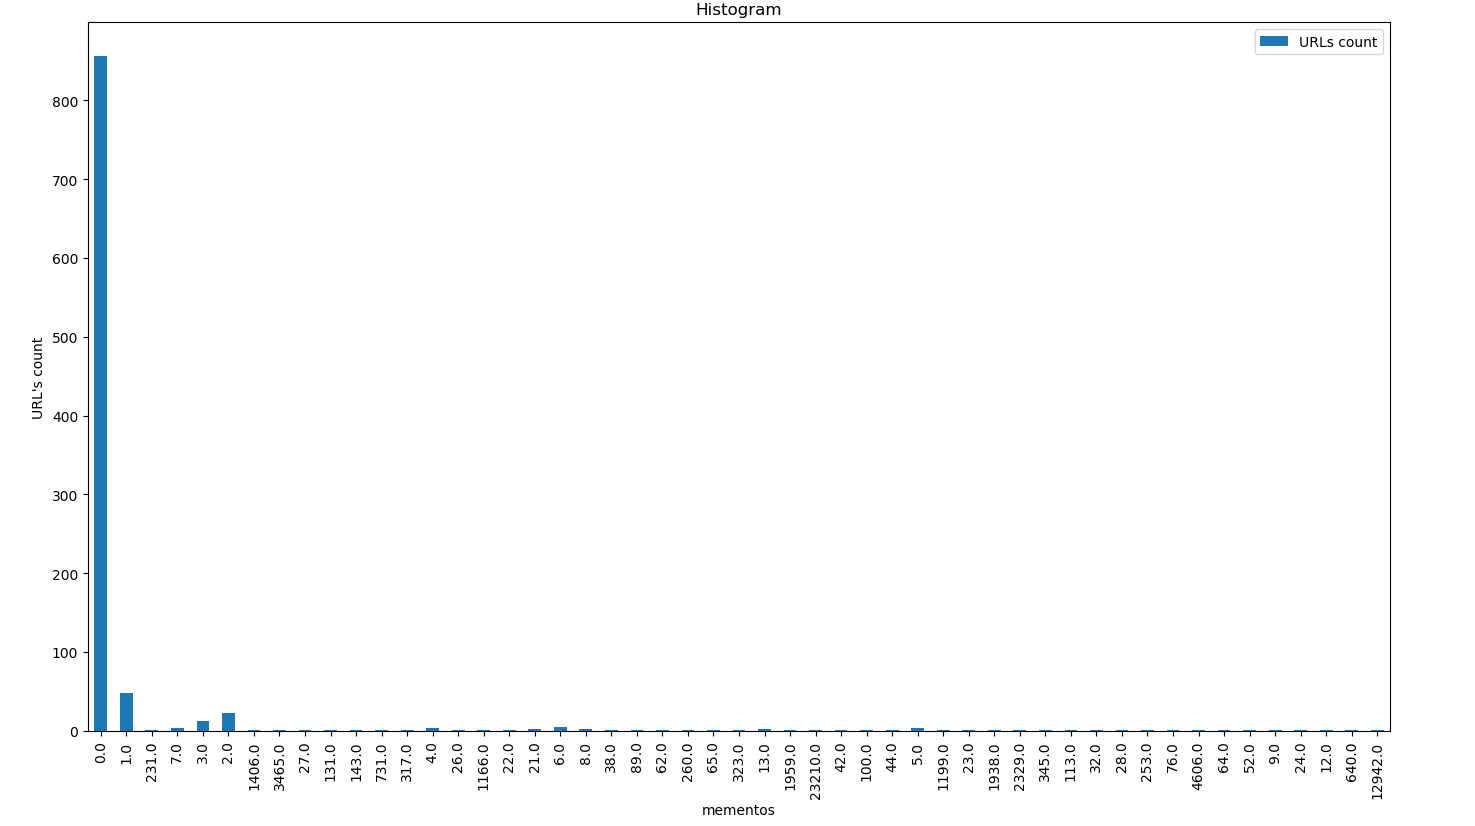
\includegraphics[scale=1.0]{histogramBarGraphImg.png}
\caption{Histogram of Number of URIs vs. Number of Mementos}
\label{fig:q2histogram}
\end{figure}
\clearpage
% =================================
% Third question
% =================================
\section*{3}
\subsection*{Question}
\begin{verbatim}
3.  Estimate the age of each of the 1000 URIs using the "Carbon
Date" tool:
http://ws-dl.blogspot.com/2016/09/2016-09-20-carbon-dating-web-version-30.html
Note: you should use "docker" and install it locally.  You can do
it like this:
http://cd.cs.odu.edu/cd?url=http://www.cs.odu.edu/
But it will inevitably crash when everyone tries to use it at the
last minute.
For URIs that have > 0 Mementos and an estimated creation date,
create a graph with age (in days) on the x-axis and number of
mementos on the y-axis.
Not all URIs will have Mementos, and not all URIs will have an
estimated creation date.  Show how many fall into either categories.
For example,
total URIs:         1000
no mementos:     137  
no date estimate:  212
\end{verbatim}
\clearpage
\subsection*{Solution}
To solve the above problem, used the carbon dating tool \cite{carbondateref} provided in the question to retrieve the estimated creation dates and memgator to fetch the number of memtos for each of the URIs from the existing  \textbf{finalurls.txt} file.In this I am getting mementos and age of the URLs.
Libraries used to find age and mementos are:
\begin{itemize}
  \item import requests
  \item import json
  \item from datetime import datetime
  \item import csv
   \item import errno
\end{itemize}  

I am passing each URL from  \textbf{finalurls.txt} to  \textbf{carbonDateAgeCalculation} function, in which carbon date and mentos are finding and writing  all URLs of age and mementos whose status_code 200 in \textbf{ageAndMementos.csv}. The program shown in Listing \textbf{carbonDate.py} was written in Python and the output was saved in \textbf{ageAndMementos.csv} while with column names as age and mementos.
 \subsection*{Run on the command line}
\begin{lstlisting}[frame=single]
python carbonDate.py
\end{lstlisting}
\lstinputlisting[frame=single,caption={Python script for finding the carbon date},label=lst:q2carbonpy,captionpos=b,numbers=left,showspaces=false,showstringspaces=false,basicstyle=\footnotesize]{carbonDate.py}
Libraries used for plotting scatter plot:
\begin{itemize}
  \item import pandas as pd
  \item import matplotlib.pyplot as plt
\end{itemize}
 \subsection*{Run on the command line}
\begin{lstlisting}[frame=single]
python ageVSmementosScatterPlot.py
\end{lstlisting}
All the values of URLs of age and mementos are stored in  \textbf{ageAndMementos.csv}. Used Python language to plot scatter graph.
\lstinputlisting[frame=single,caption={Python script for scatter graph},label=lst:q2carbonpy,captionpos=b,numbers=left,showspaces=false,showstringspaces=false,basicstyle=\footnotesize]{ageVSmementosScatterPlot.py}
\begin{figure}[h]
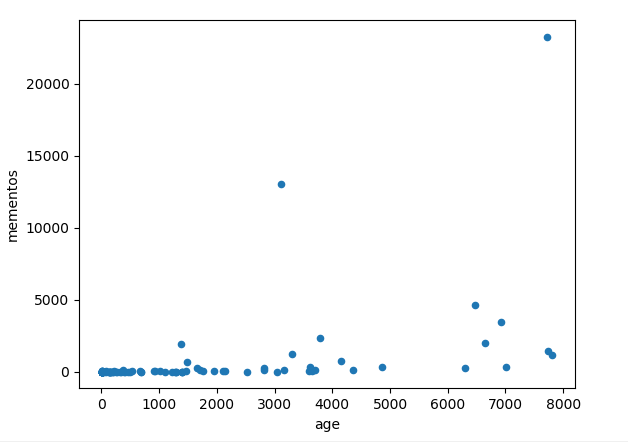
\includegraphics[scale=1.0]{ageVSmemntosScatterPlotGraph.png}
\caption{Scatter plot of age in days and number of mementos}
\label{fig:scatterplot}
\end{figure}
Also the program in Listing,  calculated the following values and saved in \textbf{ageOfGoodLinks.txt} file.
\begin{itemize}
  \item total URIs:	     1001
  \item no mementos:      846
  \item no date estimate: 139
\end{itemize}

\clearpage
% =================================
% Bibliography
% =================================
\begin{thebibliography}{9}
\bibitem{twitterref}
Python Programmng. ``Twitter API Streaming.''  N.p., 13 Feb. 2018.\url{https://pythonprogramming.net/twitter-api-streaming-tweets-python-tutorial/}
\bibitem{streamref} 
Tweepy Documentation. ``Tweepy Documentation - tweepy 3.5.0 .''  N.p., 13 Feb. 2018. \url{http://docs.tweepy.org/en/v3.5.0/index.html}
\bibitem{tlderef} 
Python Software Foundation. ``tldextract 2.2.0 : Python Package Index .''  N.p., 13 Feb. 2018. \url{https://pypi.python.org/pypi/tldextract}
\bibitem{jsonref} 
Python Software Foundation. ``19.2. json - JSON encoder and decoder - Python 3.6.4 documentation .''  N.p., 13 Feb. 2018. \url{https://docs.python.org/3/library/json.html}
\bibitem{csvref} 
Python Software Foundation. ``14.1. csv - CSV File Reading and Writing - Python 3.6.4 documentation.''  N.p., 13 Feb. 2018. \url{https://docs.python.org/3/library/csv.html}
\bibitem{parseref} 
Urllib.parse Documentation. ``21.8. urllib.parse — Parse URLs into components — Python 3.6.4 documentation, Web. 13 Feb. 2018. \url{https://docs.python.org/3/library/urllib.parse.html}
\bibitem{urllibref} 
 Urllib.requests Documentation.``Developer Interface — Requests 2.18.4 documentation", Web. 13 Feb, 2018. \url{https://docs.python.org/3.0/library/urllib.request.html}

\end{thebibliography}
\end{document}